
\chapter{Background}

\section{Theory Overview}
In this thesis we are trying to extract features from a given dataset in order to perform a Logistic Regression and predict missing or future links. 





\subsection{Feature Extraction}
Full definition taken from wikipedia (en.wikipedia.org/wiki/Feature\_extraction): 
\begin{quote} 
In machine learning, pattern recognition and in image processing, feature extraction starts from an initial set of measured data and builds derived values (features) intended to be informative and non-redundant, facilitating the subsequent learning and generalization steps, and in some cases leading to better human interpretations. Feature extraction is related to dimensionality reduction.

When the input data to an algorithm is too large to be processed and it is suspected to be redundant (e.g. the same measurement in both feet and meters, or the repetitiveness of images presented as pixels), then it can be transformed into a reduced set of features (also named a feature vector). Determining a subset of the initial features is called feature selection.[1] The selected features are expected to contain the relevant information from the input data, so that the desired task can be performed by using this reduced representation instead of the complete initial data.
\end{quote}
\subsection{Logistic Regression}
Full definition taken from Research methods inhuman skeletal biology[2]: 
\begin{quote} 
Logistic regression (LR) is a statistical method similar to linear regression since LR finds an equation that predicts an outcome for a binary variable, Y, from one or more response variables, X. However, unlike linear regression the response variables can be categorical or continuous, as the model does not strictly require continuous data. To predict group membership, LR uses the log odds ratio rather than probabilities and an iterative maximum likelihood method rather than a least squares to fit the final model. This means the researcher has more freedom when using LR and the method may be more appropriate for nonnormally distributed data or when the samples have unequal covariance matrices. Logistic regression assumes independence among variables, which is not always met in morphoscopic datasets. However, as is often the case, the applicability of the method (and how well it works, e.g., the classification error) often trumps statistical assumptions. One drawback of LR is that the method cannot produce typicality probabilities (useful for forensic casework), but these values may be substituted with nonparametric methods such as ranked probabilities and ranked interindividual similarity measures. 
\end{quote}

\section{Tools Overview}
The project was created using Java and Apache-Flink. We build the project using Apache Maven. 

\subsection{Apache Flink}
All information were taken from Apache Flink Website: 
\begin{quote}
Apache Flink is a framework and distributed processing engine for stateful computations over unbounded and bounded data streams, designed to run in all common cluster environments and perform computations at in-memory speed and at any scale.
    \begin{description}
    \item $\bullet$ Unbounded streams have a start but no defined end. They must be continuously processed and it is not possible to wait for all input data to arrive.
    \item $\bullet$ Bounded streams have a defined start and end. Bounded streams can be processed by ingesting all data before performing any computations. Processing of bounded streams is also known as batch processing.
    \end{description}
    
Apache Flink excels at processing unbounded and bounded data sets. Precise control of time and state enable Flink’s runtime to run any kind of application on unbounded streams. Bounded streams are internally processed by algorithms and data structures that are specifically designed for fixed sized data sets, yielding excellent performance.


Apache Flink is a distributed system and requires compute resources in order to execute applications. Flink integrates with all common cluster resource managers such as Hadoop YARN, Apache Mesos, and Kubernetes but can also be setup to run as a stand-alone cluster.It is designed to work well each of the previously listed resource managers. This is achieved by resource-manager-specific deployment modes that allow Flink to interact with each resource manager in its idiomatic way.


When deploying a Flink application, Flink automatically identifies the required resources based on the application’s configured parallelism and requests them from the resource manager. In case of a failure, Flink replaces the failed container by requesting new resources. All communication to submit or control an application happens via REST calls. This eases the integration of Flink in many environments.


Flink is designed to run stateful streaming applications at any scale. Applications are parallelized into possibly thousands of tasks that are distributed and concurrently executed in a cluster. Therefore, an application can leverage virtually unlimited amounts of CPUs, main memory, disk and network IO. Moreover, Flink easily maintains very large application state. Its asynchronous and incremental checkpointing algorithm ensures minimal impact on processing latencies while guaranteeing exactly-once state consistency.


Stateful Flink applications are optimized for local state access. Task state is always maintained in memory or, if the state size exceeds the available memory, in access-efficient on-disk data structures. Hence, tasks perform all computations by accessing local, often in-memory, state yielding very low processing latencies. Flink guarantees exactly-once state consistency in case of failures by periodically and asynchronously checkpointing the local state to durable storage.

\end{quote}
\subsection{Apache Maven}
All information were taken from Apache Maven website: 
\begin{quote}

Maven began as an attempt to simplify the build processes in the Jakarta Turbine project. There were several projects, each with their own Ant build files, that were all slightly different. JARs were checked into CVS. They needed a standard way to build the projects, a clear definition of what the project consisted of, an easy way to publish project information, and a way to share JARs across several projects.
The result is a tool that can now be used for building and managing any Java-based project. 

Maven’s primary goal is to allow a developer to comprehend the complete state of a development effort in the shortest period of time. In order to attain this goal, Maven deals with several areas of concern:
   \begin{description}
    \item $\bullet$Making the build process easy
   \item $\bullet$ Providing a uniform build system
    \item $\bullet$Providing quality project information
    \item $\bullet$Encouraging better development practices
      \end{description}



While using Maven doesn’t eliminate the need to know about the underlying mechanisms, Maven does shield developers from many details. It builds a project using its project object model (POM) and a set of plugins. Maven provides useful project information that is in part taken from your POM and in part generated from your project’s sources. For example, Maven can provide:
    \begin{description}
    \item $\bullet$Change log created directly from source control
    \item $\bullet$Cross referenced sources
    \item $\bullet$Mailing lists managed by the project
    \item $\bullet$Dependencies used by the project
    \item $\bullet$Unit test reports including coverage
     \end{description}
Third party code analysis products also provide Maven plugins that add their reports to the standard information given by Maven.

\end{quote}
%\section{A Section that Contains Some Maths}

  % Replace with your text
 
%\begin{equation}
%M = \frac{1}{T}\sum_{t=1}^{T} e(t) / \max_{t}[e(t)]
%\label{eq:equation}
%\end{equation}

  % Replace with your text

%This is shown in Equation \ref{eq:equation} and is repeated here $M = \frac{1}{T}\sum_{t=1}^{T} e(t) / \max_{t}[e(t)]$.


%\section{A Section that Contains a Figure}

  % Replace with your text

%\begin{figure}[ht]
%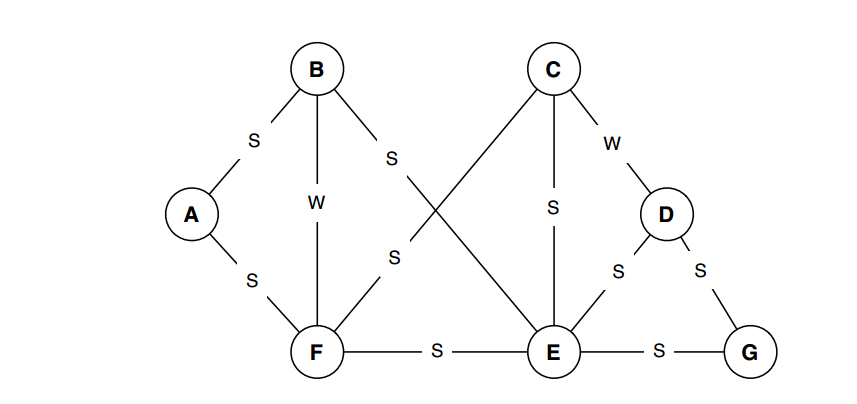
\includegraphics[width=15cm]{figures/figure1.png}
%\caption{A simple figure in \LaTeX. Reproduced from http://tinyurl.com/nqtrlj5 with the permission of the %copyright owner.}
%\label{fig:graph}
%\end{figure}

% Replace with your text

%See Figure \ref{fig:graph}.


%\section{A Section that Contains a Table}

  % Replace with your text

%\begin{table}[ht]
%\center
%\begin{tabular}{cc|c}
%A & B & A XOR B\\
%\hline
%0 & 0 & 0\\
%0 & 1 & 1\\
%1 & 0 & 1\\
%1 & 1 & 0\\
%\end{tabular}
%\caption{A simple table in \LaTeX.}
%\label{tab:xor}
%\end{table}
 % Replace with your text

%This is shown in Table \ref{tab:xor}.




 % Replace with your text
